\cleardoublepage

\chapter{Propuesta}
\label{ch:Capitulo3}

Tras presentar diferentes tecnologías, software, protocolos de comunicación y hardware planteados en el ámbito de la domótica del hogar del capitulo Chapter~\ref{ch:Capitulo2}, en la búsqueda de una solución libre y de bajo coste, que pueda alcanzar los objetivos planteados para la creación de un prototipo de suite domótica, se propone:

\vspace{1cm}

Desarrollar un prototipo de suite domótica que opere en una red local inalámbrica cuyo router actúe como nodo principal, ejecutado en un ordenador de bajo consumo, que permita la interconexión para dispositivos inalámbricos con roles de actuadores o sensores. Además, debe ser posible operar dicha suite, desde dentro de la red local en la que opera el nodo, o desde fuera de la misma mediante conexiones remotas cifradas, mediante una aplicación para dispositivo móvil con sistema operativo Android. Si bien, la operatividad remota es opcional, se debe alcanzar la gestión de la suite en el entorno de la red local, cumpliendo así con el objetivo de disponer de un sistema aislado y autónomo, que no dependa de servicios externos para su funcionamiento. Una vez alcanzada una implementación funcional del prototipo se aplicará en dos casos de usos que ejemplifican la entrada y salidas características de todo sistema de domótica, la recepción, proceso y presentación de datos de un dispositivo sensor en la aplicación móvil, y la gestión de un actuador desde dicha aplicación. Esta suite debe cubrir la necesidad de controlar el estado de una bodega de uso personal en una casa, pudiendo obtener valores ambientales de la estancia y controlar el sistema de iluminación de la escalera que accede a la misma, pudiendo alternar el estado de las luces de manera automática o manualmente, desde la aplicación.


Se ha elegido no utilizar un \gls{framework} concreto para el desarrollo de nuestra suite domótica. Si bien, no utilizaremos \gls{framework} orientados a domotica, pero si se utilizaran \gls{framework} de servicios [INCLUIR AQUI ANGULAR, IONIC y NODE]. Es necesario determinar el conjunto de servicios bajo el cual operará nuestra solución domótica.


\section{Módulos de la propuesta}
\label{ch:Capitulo3.1}
Para lograr la propuesta, será necesario considerar de entre las opciones estudiadas en el  Chapter~\ref{ch:Capitulo2} aquellas que se ajustan mejor al alcance de esta propuesta. Dadas las distintas capas de hardware, arquitectura de red y software que componen este proyecto, la propuesta será dividida en tres conceptos modulares, permitiendo un desarrollo individual y en paralelo respecto de cada uno.

\begin{itemize}

\item Se creará un nodo principal que actuara como router de la red de dispositivos de la suite domótica y servidor de la aplicación móvil. Dispondrá de la capacidad de ser operado de forma remota o local, almacenara los servicios y aplicaciones necesarios para que funcione la suite domótica ejecutándose en un ordenador de bajo consumo.

\item Se genera distintos dispositivos sensores o actuadores que podrán incluirse en la red inalámbrica del nodo principal y podrán ser operados desde dicho nodo.

\item Y por último la aplicación movil (front-end) y servidor (back-end) que darán al usuario la capacidad de gestionar la suite domótica.

\end{itemize}

\section{Módulo de Gateway}
\label{ch:Capitulo3.2}

Se tratará de alcanzar una cierta descentralización de los dispositivos y la propia Raspberry, basándose en el concepto de nodo principal (gateway), que habitualmente se observa en las plataformas de pago.

Dichos planteamientos se basan en que todo sensor/actuador que forme parte de red de dispositivos de una solución de domótica actual, es gestionada a través de un nodo. En vez de conectar los dispositivos inalámbricos a el router de la casa, se conectan al nodo y este, a su vez, es quien se conecta a la red local del hogar, para así conectarse con los servicios externos. En general, las distintas plataformas has alcanzado un acuerdo no formalizado de actuación que funciona de la siguiente forma. El usuario final compra un nuevo dispositivo, lo enciende, dejándolo en un estado de "inclusión" a la red domótica, después, desde la aplicación de móvil, se indica al nodo, que se quiere añadir un nuevo dispositivo, y tras seguir las indicaciones, el dispositivo se registra en la red del nodo. Esto, sin embargo, tiene algunos inconvenientes en el proceso de "inclusión", y aunque la probabilidad es baja, puede suceder que dos nodos de distintas viviendas, que están registrando dispositivos simultáneamente, terminasen, registrando un dispositivo que no les corresponde. Esto es una vulnerabilidad de seguridad grave y una vertiente adicional que incluir en las motivaciones del estudio y desarrollo de una suite domótica libre que permita nuevas formulas de funcionamiento.

Se ha planteado este problema, junto con las 3 motivaciones principales, para crear un proceso de "inclusión" de dispositivos al nodo, que parta de una conexión alámbrica (vía USB) y resuelva este inconveniente, y simplifique el proceso de las soluciones privadas, que en ocasiones pueden fallar.

\vspace{1cm}


\section{Módulo de dispositivos \gls{iot}}
\label{ch:Capitulo3.3}


\section{Módulo de dispositivos \gls{iot}}
\label{ch:Capitulo3.4}


\section{Módulo de front-End y back-end}
\label{ch:Capitulo3.5}

\section{Propuesta de casos de uso}
\label{ch:Capitulo3.6}

El primer caso de uso consistirá en una simple interacción del usuario con la suite domótica para consultar la temperatura y/o humedad de una estancia. Para ello, es necesario disponer de un dispositivo inalámbrico con un sensor que recoja las mediciones y puedan ser mostradas al usuario en su smartphone.

El segundo caso de uso cubrirá la gestión por parte del usuario de un actuador basado en un interruptor de corriente, pudiendo consultar su estado actual y alternar dicho estado, también desde un smartphone.

\section{Objetivos adicionales}
\label{ch:Capitulo3.7}

Las siguientes propuestas corresponden más a un declaración de intenciones que a objetivos necesarios para cumplir la propuesta del proyecto. Son un valor añadido y deseable siempre que no comprometan los plazos de tiempo marcados por la entrega final de este documento al director de proyecto. Se encuentran enumerados según el valor de importancia.

\begin{enumerate}

  \item Vinculación de dispositivos con la red de suite domótica mediante USB, en lugar del clásico emparejamiento WIFI.

  \item Creación de una imagen autoinstalable de para otros usuarios

  \item Integración de múltiples opciones de hardware compatibles con la suite domótica.

  \item Conexiones cifradas en la red de dispositivos y en la comunicación entre aplicación movil y servidor.

  \item Exportar la suite domótica en una imagen autoinstalable, de fácil instalación que permita replicar el prototipo creado.

\end{enumerate}

\begin{figure}[hbt!]
\centering
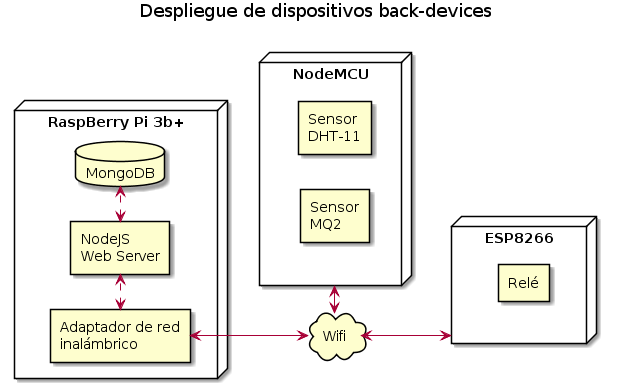
\includegraphics[height=2.5in]{figures/diagrams/physical-devices/back-devices.png}
\caption[back-devices]{back-devices\footnotemark}
\end{figure}

\begin{figure}[hbt!]
\centering
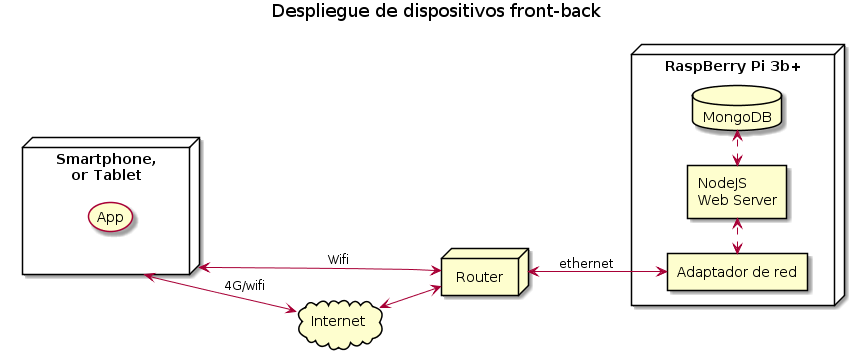
\includegraphics[height=2.5in]{figures/diagrams/physical-devices/front-back.png}
\caption[front-back]{front-back\footnotemark}
\end{figure}

\begin{figure}[hbt!]
\centering
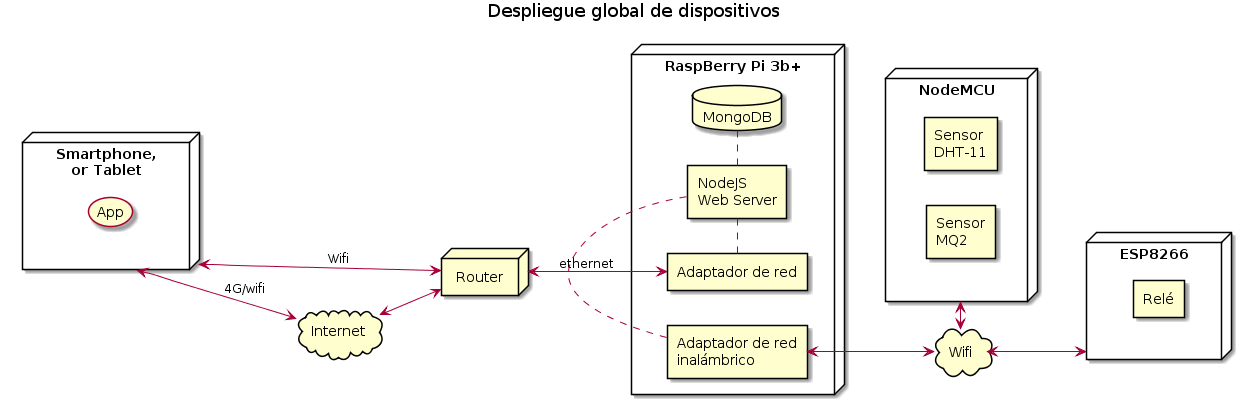
\includegraphics[height=2.5in]{figures/diagrams/physical-devices/global.png}
\caption[global]{global\footnotemark}
\end{figure}

\begin{figure}[hbt!]
\centering
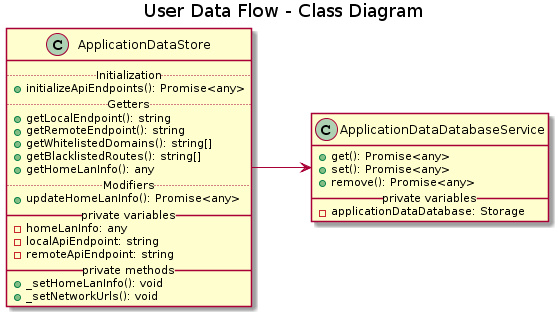
\includegraphics[height=2.5in]{figures/diagrams/front/data-flow/app-data.png}
\caption[app-data]{app-data\footnotemark}
\end{figure}

\begin{figure}[hbt!]
\centering
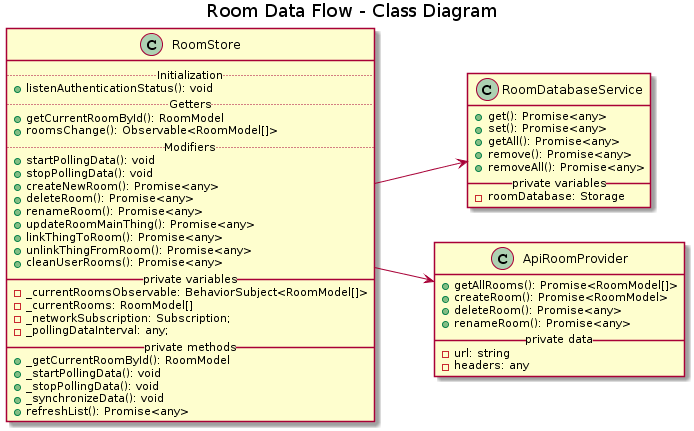
\includegraphics[height=2.5in]{figures/diagrams/front/data-flow/room.png}
\caption[room]{room\footnotemark}
\end{figure}

\begin{figure}[hbt!]
\centering
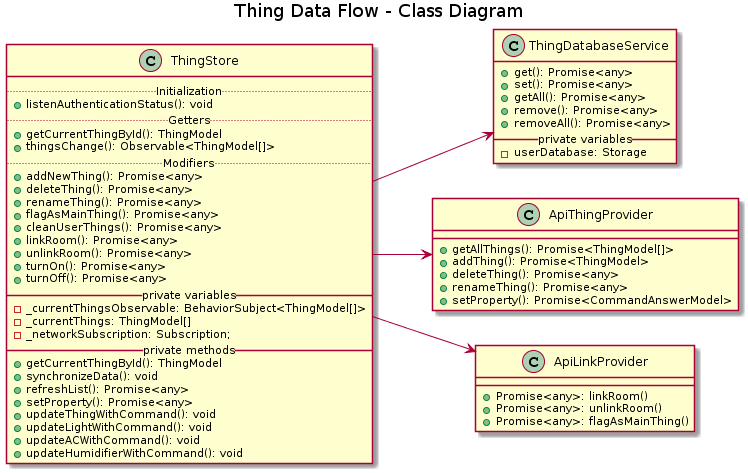
\includegraphics[height=2.5in]{figures/diagrams/front/data-flow/thing.png}
\caption[thing]{thing\footnotemark}
\end{figure}

\begin{figure}[hbt!]
\centering
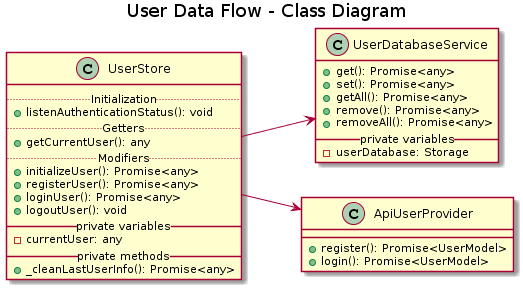
\includegraphics[height=2.5in]{figures/diagrams/front/data-flow/user.png}
\caption[user]{user\footnotemark}
\end{figure}

\begin{figure}[hbt!]
\centering
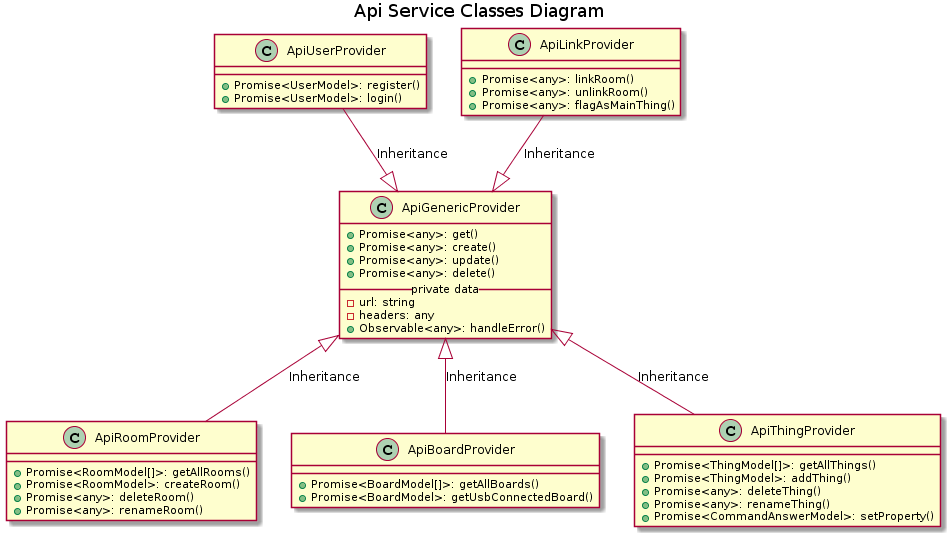
\includegraphics[height=2.5in]{figures/diagrams/front/architecture/api-services.png}
\caption[api-services]{api-services\footnotemark}
\end{figure}

\begin{figure}[hbt!]
\centering
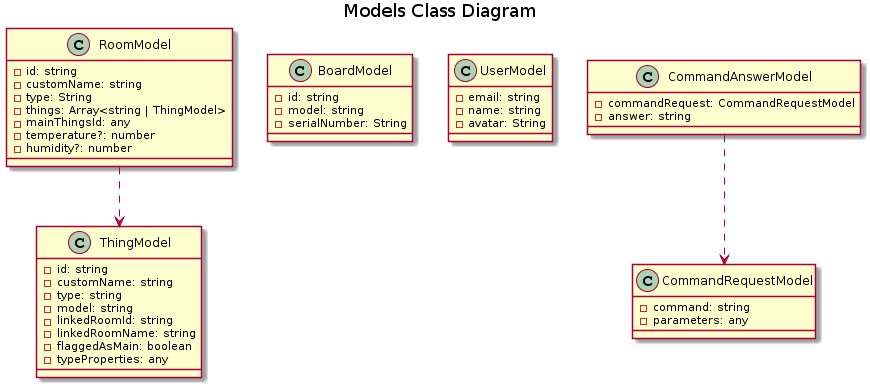
\includegraphics[height=2.5in]{figures/diagrams/front/architecture/models.png}
\caption[models]{models\footnotemark}
\end{figure}

\begin{figure}[hbt!]
\centering
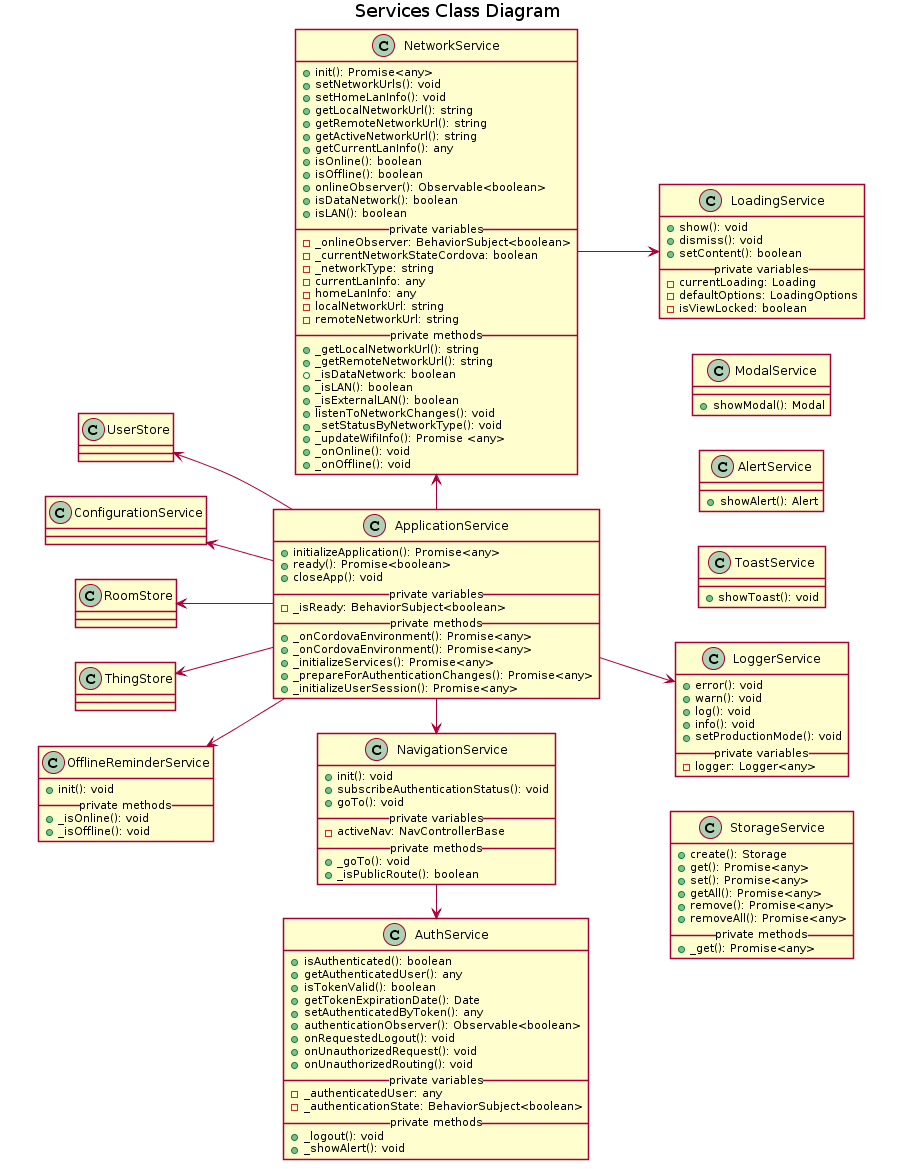
\includegraphics[height=2.5in]{figures/diagrams/front/architecture/services.png}
\caption[services]{services\footnotemark}
\end{figure}

\begin{figure}[hbt!]
\centering
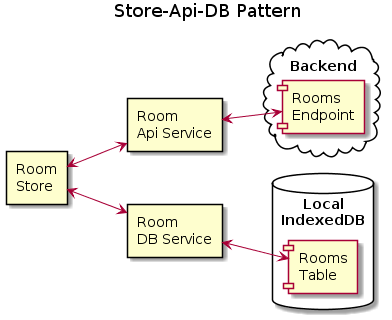
\includegraphics[height=2.5in]{figures/diagrams/front/architecture/store-api-db-pattern.png}
\caption[store-api-db-pattern]{store-api-db-pattern\footnotemark}
\end{figure}

\begin{figure}[hbt!]
\centering
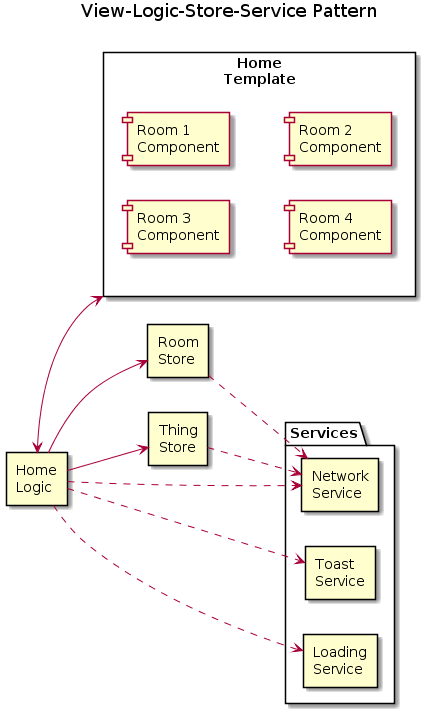
\includegraphics[height=2.5in]{figures/diagrams/front/architecture/view-logic-store-service-pattern.png}
\caption[view-logic-store-service-pattern]{view-logic-store-service-pattern\footnotemark}
\end{figure}

\begin{figure}[hbt!]
\centering
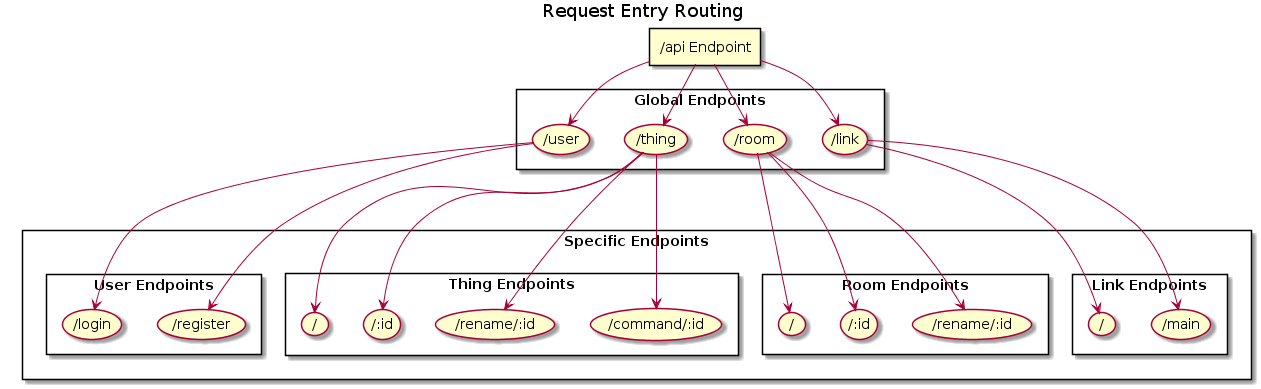
\includegraphics[height=2.5in]{figures/diagrams/back/router-flow/api-entry.png}
\caption[api-entry]{api-entry\footnotemark}
\end{figure}

\begin{figure}[hbt!]
\centering
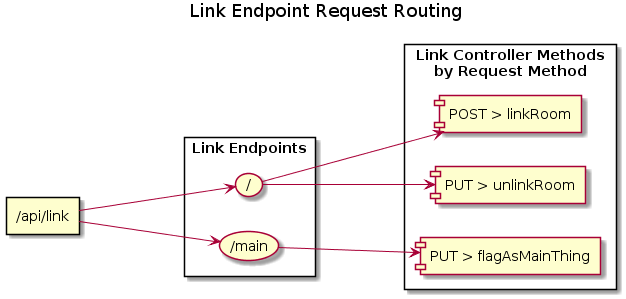
\includegraphics[height=2.5in]{figures/diagrams/back/router-flow/link-endpoints.png}
\caption[link-endpoints]{link-endpoints\footnotemark}
\end{figure}

\begin{figure}[hbt!]
\centering
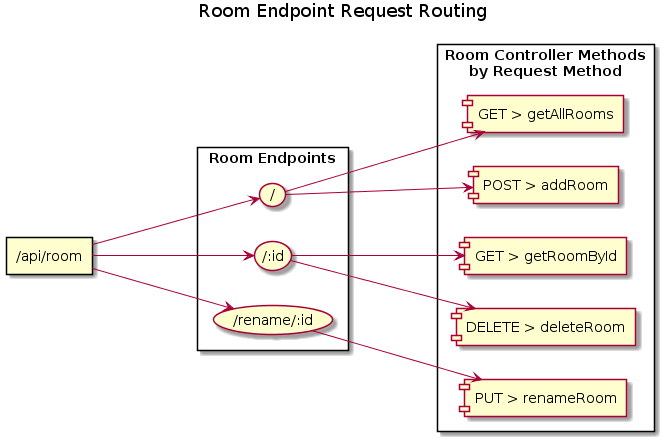
\includegraphics[height=2.5in]{figures/diagrams/back/router-flow/room-endpoints.png}
\caption[room-endpoints]{room-endpoints\footnotemark}
\end{figure}

\begin{figure}[hbt!]
\centering
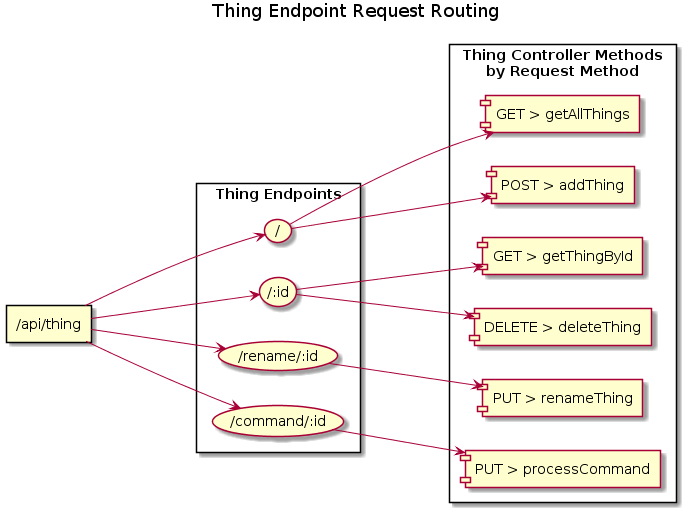
\includegraphics[height=2.5in]{figures/diagrams/back/router-flow/thing-endpoints.png}
\caption[thing-endpoints]{thing-endpoints\footnotemark}
\end{figure}

\begin{figure}[hbt!]
\centering
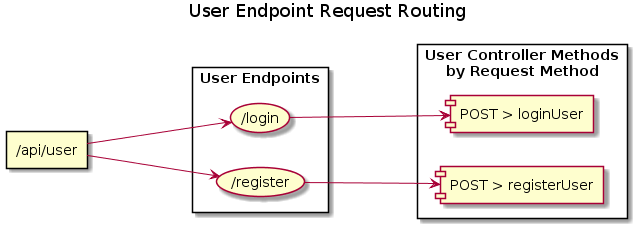
\includegraphics[height=2.5in]{figures/diagrams/back/router-flow/user-endpoints.png}
\caption[user-endpoints]{user-endpoints\footnotemark}
\end{figure}
